\documentclass[times, utf8, seminar]{fit}

%\batchmode
%\usepackage{booktabs}
\usepackage{listings}
\usepackage{longtable}
\usepackage{xcolor}
\usepackage{float}
\usepackage{enumitem}
\usepackage{hyperref}
\usepackage{enumerate}
\usepackage{graphicx}
\usepackage{etoolbox}

\begin{document}

\title{Projekat: Unapređenje informacionog sistema na primjeru jedne kompanije}

\author{Ernad Husremović}
\brindex{DL 2792}
\verzija {1.0.0}

\mentor{prof.dr Murat Prašo}

\maketitle

\tableofcontents

\listoftables
\listoffigures

% abstract begin
\begin{sazetak}


Sažetak na bosanskom jeziku.

\kljucnerijeci{bosanska rijec 1, bosanska rijec 2}
\end{sazetak}

\engtitle{Naslov na engleskom jeziku}
\begin{abstract}
Abstract na engleskom jeziku.

\keywords{key1, key2, key3}
\end{abstract}

% abstract end

\chapter{Uvod}

\section{Legalizacija - bezpovratne promjene na IT tržištu BiH}

Akcije državnih inspekcijskih organa na suzbijanju nelegalnog softvera (nadalje legalizacija) sa početkom 2012 godine označila je početak krupnih promjena na tržištu informatičkih \engl{information technology, nadalje IT} rješenja u Bosni i Hercegovini. 
Većina poslovnih subjekata koja se u proteklim godinama opremila "jeftinim" nelegalnim softverom \engl{software} našla se u nezavidnoj situaciji.
Usljed visokih troškovima legalizacije "Microsoft" softvera\footnote{familija "Microsoft Windows" OS-ova, uz svuda prisutni ali i redovno nelegalno instalirani "Microsoft Office" uredski paket}, pojavila se potražnja za softverom drugih proizvođača.  

\section{OSS software}

Preduzeće "bring.out"\footnote{\url{http://www.bring.out.ba/}} je dugi niz godina orjentisano na ponudu sistema baziranih na software-u otvorenog koda \engl{open source software, nadalje OSS}.

Potražnja za Linux/Ubuntu serverskim rješenjima \footnote{\url{http://linux.com}, \url{http://ubuntu.com}}) je postojala i prije legalizacije. Međutim, tek nakon legalizacije pojavila se potražnja za cjelovitim informatičkim IT rješenjima baziranim na OSS-u:
\begin{itemize}
  \item server operativni sistem (nadalje OS)
  \item desktop operativni sistem
  \item aplikativni softver
  \begin{itemize}
    \item opći software za uredske potrebe
    \item poslovni - softver \engl{Enterprise Resource Planning, nadalje ERP}
  \end{itemize}
\end{itemize}

\subsection{Ubuntu Linux}
"Ubuntu" Linux distribucija radi svoje jednostavnosti i kvaliteta postao popularan desktop OS.

Za razliku od "Windows" operativnih sistema, "Ubuntu" desktop sistem sadrži kompletan set aplikacija za svakodnevne potrebe:
\begin{itemize}
  \item LibreOffice uredski paket za pravljenje tekstualnih i tabelarnih dokumenata, prezentacija i crteža\footnote{U funkcionalnom smislu sličan "Microsoft office" setu aplikacija. Može obrađivati većinu "Microsoft office" dokumenata}
  \item "Inkscape", program za vektorsku grafiku \cite{inkscape}
  \item "GIMP", program za bitmapiranu grafiku
  \item "Evince", preglednik PDF dokumenata
  \item "Firefox", "Chromium" internet pretraživači
  \item "OpenProj", program za izradu i praćenje projekata\footnote{U funkcionalnom smislu sličan "Microsoft project" aplikaciji}
\end{itemize}  

 
\subsection{Razlike između otvorenog i zatvorenog softvera} 

S obzirom da su za ovaj projekat najbitniji fokus poređenja će biti "Windows" i "Ubuntu" OS. 

Lista iz predhodne sekcije predstavlja djelimičnu listu dostupnih aplikacija. Međutim, i to je dovoljno da se uoči bitna razlika između "Windows" i "Ubuntu" OS-a. 

Uz "Windows" se isporučuje samo operativni sistem, dok "Ubuntu" kao i ostale linux distribucije isporučuju kompletan sistem koji korisnik može odmah početi koristiti.

U ranom stadiju razvoja OSS softver je manjkao sa kvalitetnom dokumentacijom. Sada to nije slučaj. 

Razvoj "open source" softvera je suštinski drugačiji u odnosu na razvoj zatvorenog sofvera. Kod zatvorenog softvera sve ključne razvojne aktivnosti i sudbina softvera nalaze se u rukama jednog proizvođača.

Kod OSS-a postoji velika uključenost zajednice korisnika \engl{community}, što omogućava da se sve komponente softvera razvijaju u skladu sa potrebama i zahtjevima zajednice. Korisnicima je na raspolaganju velika količina dokumentacije koja se takođe razvija na principima otvorenosti.

Korisik ubuntu sistema na raspolaganju ima odličnu dokumentaciju za serverske \cite{ubuntudesktop} i desktop \cite{ubuntuserver}.

Zahvaljujući otvorenosti, lokalizacija programa i korisničke dokumentacije (prevod i prilagodbe za lokalno tržipte) za OSS nije vođena samo komercijalnim motivima. U mnogim zemljama postoje jake zajednice korisnika koje lokalizaciju "open source" softvera vrše na bazi volonterizma. Kako se radi o projektima od velikog javnog značaja, te zajednice su često finansirane od strane države.

Svijetli primjeri država u regionu kojima postoje jake zajednice FOSS \engl{Free and open source software} i OSS  korisnika su Makedonija i Slovenija.

Na žalost, Bosna i Hercegovina, kao i u većini stvari, na tom planu zaostaje. 

\subsection{F18 knowhowERP software}
Pored standardnih komponentni "Ubuntu" OS-a, za ERP softver će se koristiti "F18" knowhowERP software.

"F18" knowhowERP\footnote{\url{http://redmine.bring.out.ba/projects/f18}} je multiplatformsko "open source" ERP rješenje, proizvod firme "bring.out".  

Predhodnik "F18" je programsko rješenje "FMK" koje se na lokalnom tržištu koristi od 1994 godine.

"F18" je softver pravljena od Bosanaca za BiH tržište. "F18" je u cjelosti domaći proizvod.

\subsection{Cjelovito OSS IT rješenje}
Na osnovu svega što je do sada izloženo, bosanskom klijentu je moguće ponuditi cjelovito OSS IT rješenje.  

Ovaj projekat će obuhvatiti instalaciju jednog takvog sistema kod klijenta.

Komparativnom analizom utvrdićemo toškove sličnog sistema baziranog na zatvorenim tehnologijama:
\begin{enumerate}[(a)]
  \item sa uključenim troškovima legalizacije postojećeg nelegalnog "Windows" OS softvera bez zamjene postojećeg ERP aplikativnog softvera
  \item sa kompletnom zamjenom kako sistemskog, tako i aplikativnog ERP softvera.  
\end{enumerate}

\section{Profil korisnika projekta}
Korisnik je mala kompanija koja se bavi trgovinom. Sa stanovišta IT-a kompanija se sastoji od:
\begin{itemize}
  \item maloprodajna mreža od 5 prodavnica
  \item centrala kompanije sa knjigovodstvom, 4 radne stanice
  \item 1 server baze podataka 
\end{itemize}

\chapter{Analiza}

\section{Analiza problema}

Povod klijentu za traženje novog rješenja je nedavna akcija legalizacije. 

Međutim, analiza je pokazala da su glavni problemi leže u činjenici da postojeći poslovni IS ne obezbjeđuje sve potrebne podatke. Već nakon prvog sastanka sa klijentom utvrđeni su sljedeći problemi, prikazani piramidom problema (\cite{prasopro}):

\begin{figure}[H]
\centering
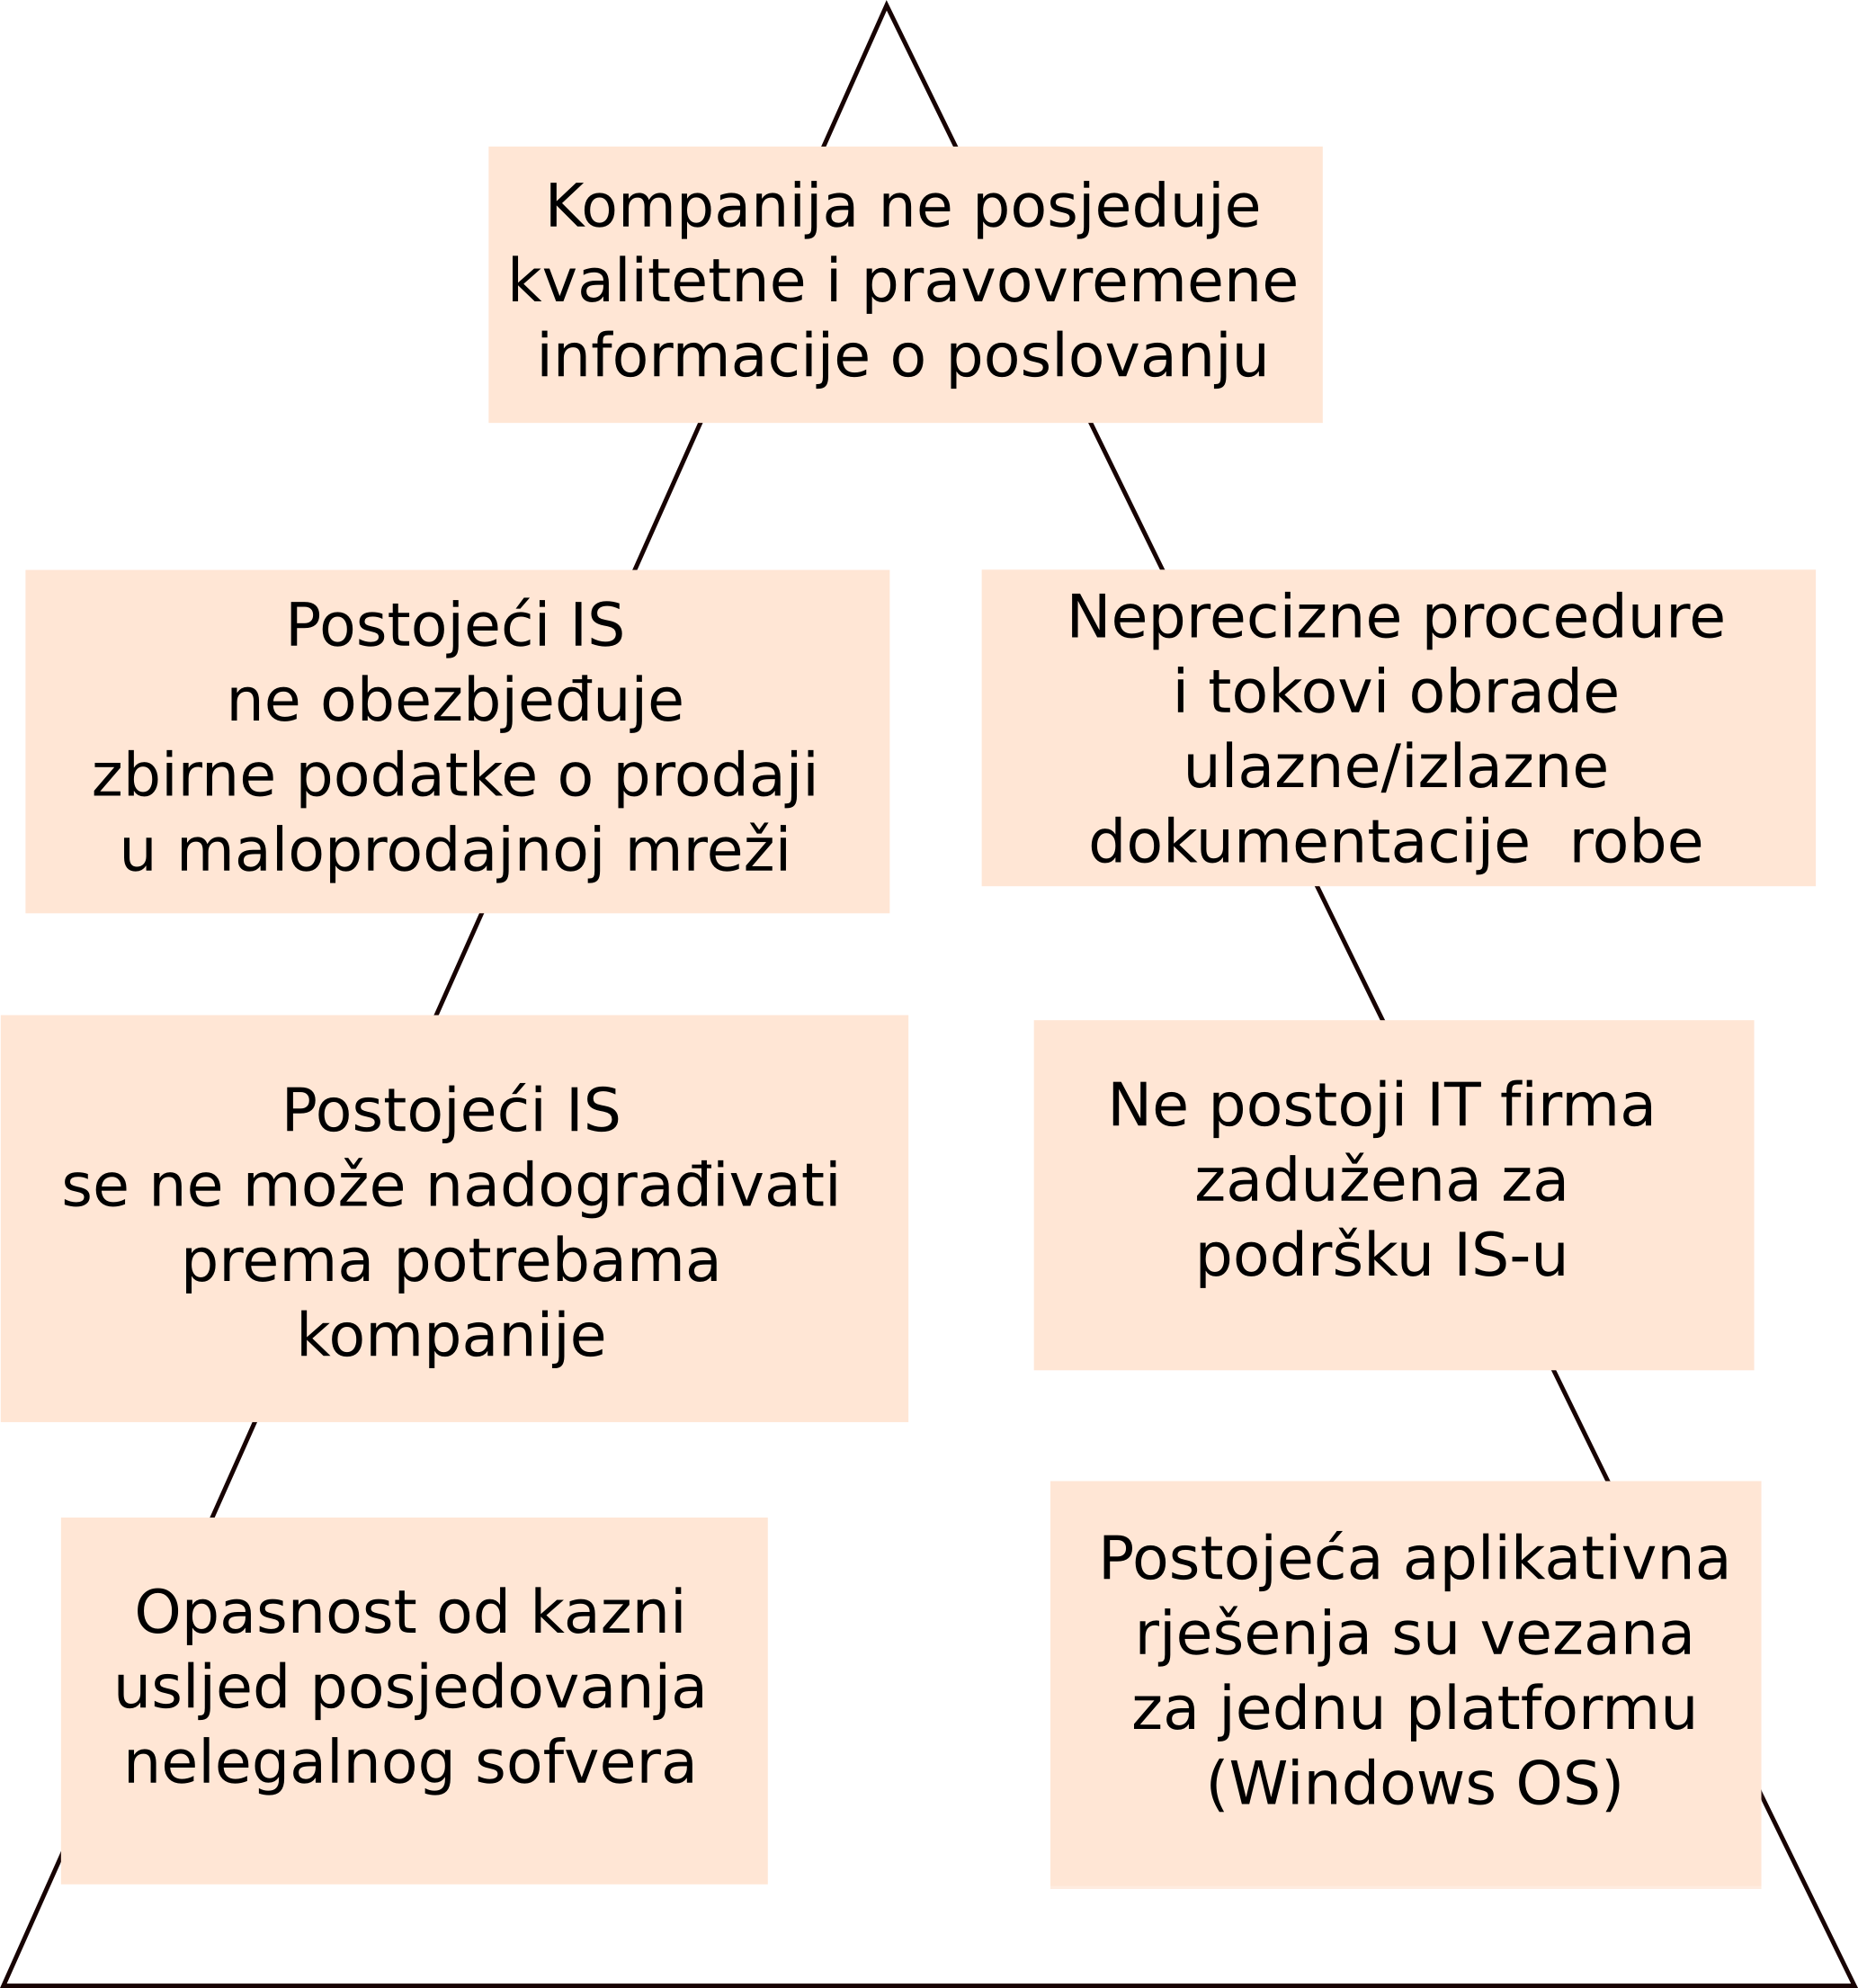
\includegraphics[width=12cm]{img/piramida_problema.png}
\caption{Piramida problema}
%\caption{bla bla (\cite{web:eric})}
\end{figure}

Piramida na vrhu prikazuje opće probleme da bi se idući ka dnu ti problemi konkretizirali.  

\section{Analiza cilja}
Analizom problema prezentovanih piramidom problema brzo dolazimo do strateškog cilja ovog projekta:
%\patchcmd{\quote}{\rightmargin}{\leftmargin 6em \rightmargin}{}{}
\begin{quote}
\em Uvođenjem novog IS-a poboljšati pravovremenost i kvalitet tekućih informacija o poslovanju.} 
\end{quote}
Analogno ranijem grafičkom prikazu problema, putem piramide ciljeva od dna ka vrhu prezentujemo ciljeve čijom realizacijom postižemo strateški cilj:

\begin{figure}[H]
\centering
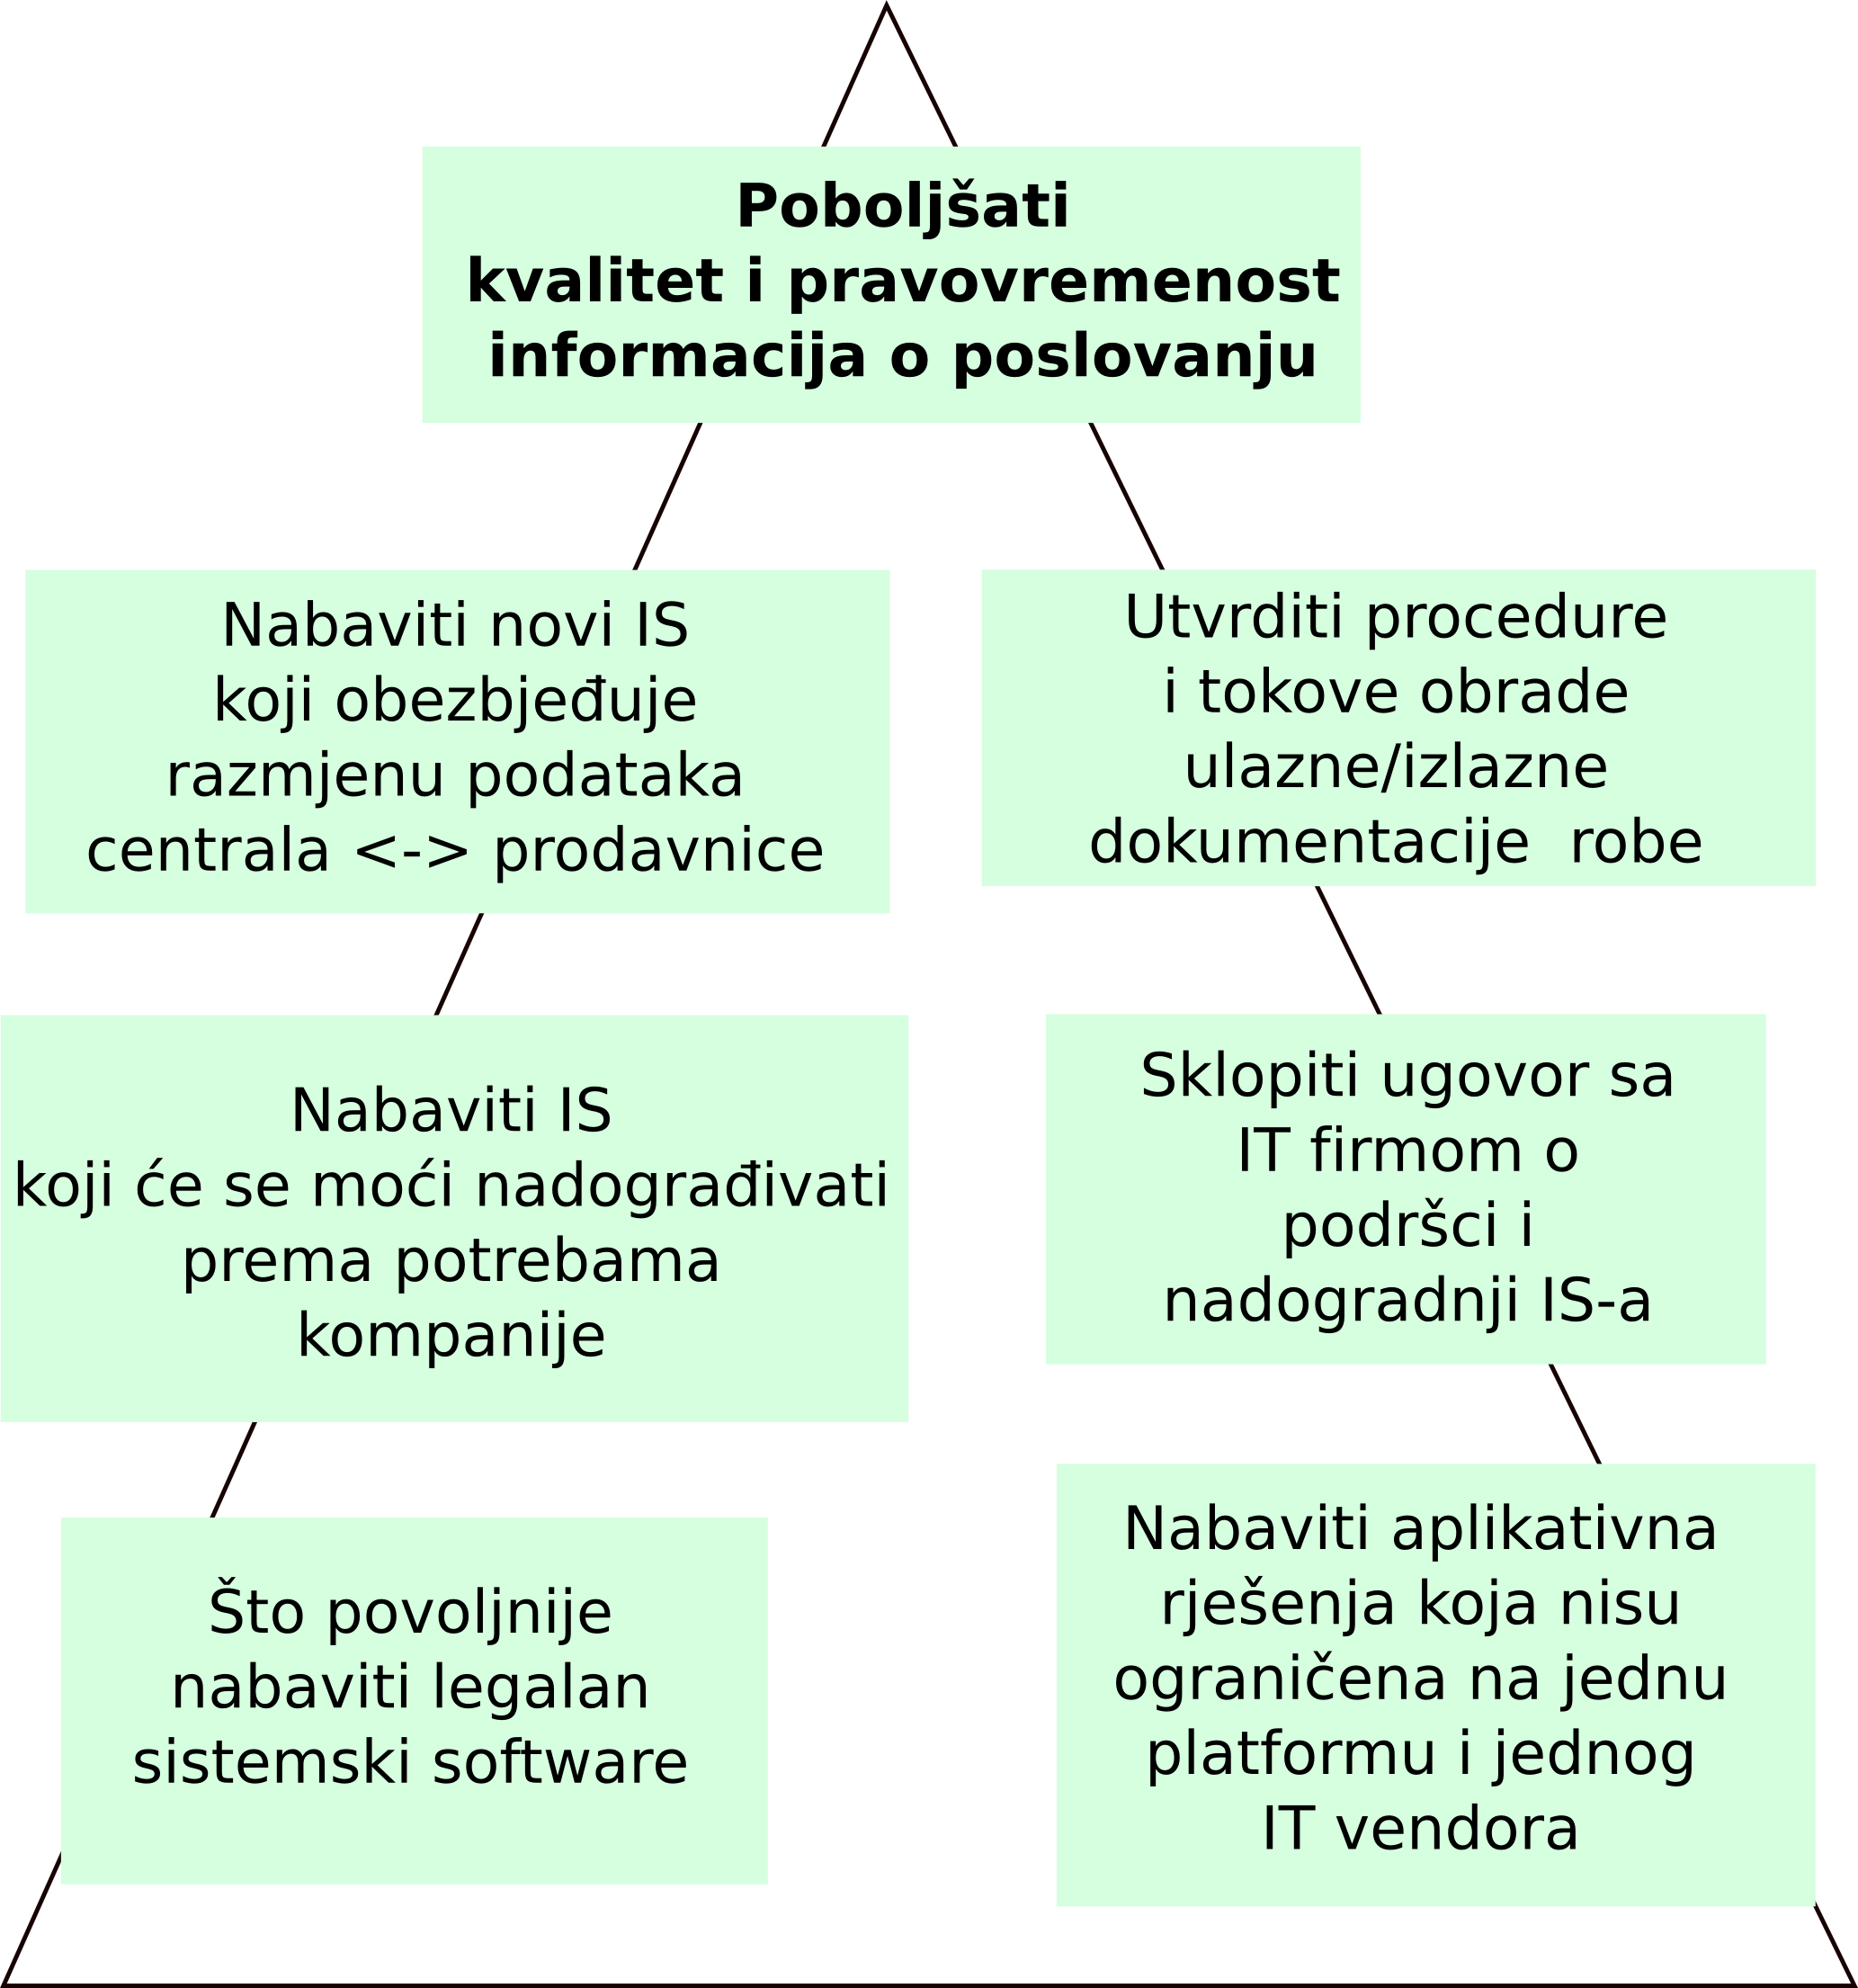
\includegraphics[width=12cm]{img/piramida_cilja.png}
\caption{Piramida cilja}
\end{figure}

\section{Logički okvir projekta}
Na kraju analize dolazimo do ključnih odrednica projekta:
\begin{table}[h]
%\centering
\resizebox{15cm}{!} {
\begin{tabular}{ | r | l | }
\hline
Svrha projekta: & Unapređenje poslovanja kompanije obezbjeđenjem kvalitetnijih informacija o poslovanju \\ \hline
Cilj: & Uvođenje novog informacionog sistema \\ \hline
Ulazi projekta: & Postojeći informacioni sistem, postojeća organizacija poslovanja \\ \hline
Izlazi projekta: & Unapređeni informacioni sistem, unapređena organizacija poslovanja \\ \hline
\end{tabular}
}

\caption{Logički okvir projekta}
\end{table}


\label{tab:myfirsttable}
\label{labela_oznaka}

\begin{description}
  \item [item 1]  objasni item 1
  \item [item 2] objasni item 2
\end{description}
 

Citacija \cite[str.~391]{pentaho32}.

\begin{itemize}
   \item vako 
   \item nako
\end{itemize}

Referenca na sekciju sekcija1 (vidi \ref{sect:sekcija1}).
 

\section{Zaključak}

\bibliography{literatura}
\bibliographystyle{fit}

\appendix

\chapter{dodatak 1}
\label{chap:dodatak1}

\chapter{Korišteni softver}

Softver korišten za realizaciju ovog dokumenta:
\begin{enumerate}
  \item Mac OS X 10.6.8
  \item Ubuntu Linux 12.04 Unity, 64bit
  \item mvim, vim tekst editor ver 7.3
  \item MacTex - pdfTeX 3.1415926-2.3-1.40.12 (TeX Live 2011)
  \item Windows XP Proffesional\footnote{kupac "bring.out" u sklopu MSDN Universal paketa, developer Ernad Husremović} on VirtualBox 4.1.16 MacOSX 
  \item Microsoft Project 2010, trial, ProductID 02252-552-2789414-37542
  \item LibreOffice 3.5.4 ?
  \item Inkscape 0.4.8, Mac OSX X11
\end{enumerate}

\begin{itemize}

\chapter{Bilješke}
\label{chap:biljeske}


\end{document}
